\begin{figure}[htbp]
    \centering
    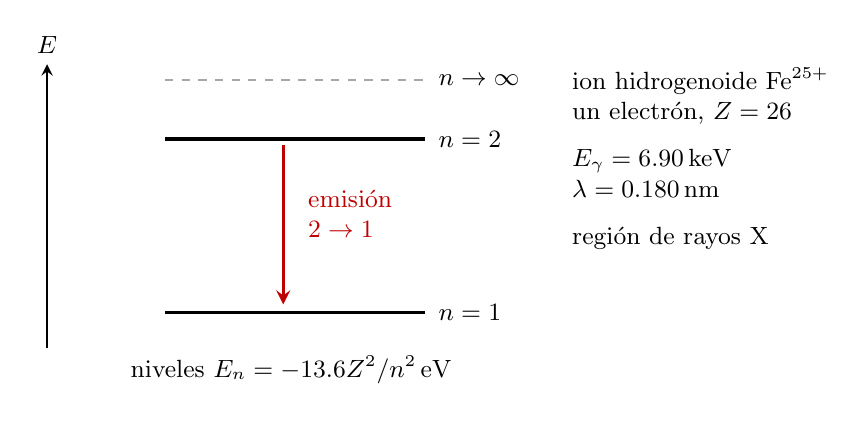
\begin{tikzpicture}[>=stealth, every node/.style={font=\small}]
        \draw[->,thick] (0,0.1) -- (0,3.7) node[above] {$E$};
        \draw[very thick] (1.5,0.55) -- (4.8,0.55);
        \draw[very thick] (1.5,2.75) -- (4.8,2.75);
        \draw[thick,dashed,gray!70] (1.5,3.5) -- (4.8,3.5);
        \node[right] at (4.85,0.55) {$n=1$};
        \node[right] at (4.85,2.75) {$n=2$};
        \node[right] at (4.85,3.5) {$n\to\infty$};
        \draw[->,very thick,red!75!black] (3.0,2.68) -- (3.0,0.65);
        \node[red!75!black,align=left] at (3.85,1.8) {emisión\\$2\to1$};
        \node[align=left] at (8.3,2.5)
            {ion hidrogenoide Fe$^{25+}$\\un electrón, $Z=26$\\[6pt]
             $E_\gamma=6.90\,\mathrm{keV}$\\
             $\lambda=0.180\,\mathrm{nm}$\\[6pt]
             región de rayos X};
        \node[below] at (3.1,0.12) {niveles $E_n=-13.6Z^2/n^2\,\mathrm{eV}$};
    \end{tikzpicture}
    \caption{Transición $n=2\to1$ del ion de hierro hidrogenoide. La diferencia de energías determina la longitud de onda; el coeficiente de Einstein $A_{21}$ determina la tasa de transición.}
    \label{fig:fe-hidrogenoide}
\end{figure}